\documentclass[11pt]{amsart}
\usepackage{geometry}                % See geometry.pdf to learn the layout options. There are lots.
\geometry{letterpaper}                   % ... or a4paper or a5paper or ... 
%\geometry{landscape}                % Activate for for rotated page geometry
%\usepackage[parfill]{parskip}    % Activate to begin paragraphs with an empty line rather than an indent
\usepackage{graphicx}
\usepackage{amssymb}
\usepackage{epstopdf}
\usepackage[usenames,dvipsnames]{color}
\usepackage{fancyvrb}
\usepackage{listings}
\usepackage{booktabs,footmisc}
\usepackage{hyperref}
\usepackage[all]{hypcap}

\usepackage{topcapt}


 
% include the lines below to use a nicer fixed-width font than the default one
 
\lstset{fancyvrb=true}
\lstset{
	basicstyle=\small\tt,
	identifierstyle=,
	commentstyle=\color{Bittersweet},
	stringstyle=\color{red},
	showstringspaces=false,
	tabsize=3,
	numbers=left,
	captionpos=b,
	xleftmargin=2em
%	numberstyle=\tiny
	%stepnumber=4
	}
\DeclareGraphicsRule{.tif}{png}{.png}{`convert #1 `dirname #1`/`basename #1 .tif`.png}

\title{Repast Simphony Batch Runs Getting Started}
\author{Nick Collier, Jonathan Ozik  - Repast Development Team}
%\date{\today}                                           % Activate to display a given date or no date

\begin{document} 
\maketitle
\setcounter{section}{-1}

\section{Before We Get Started}
Before we can do anything with Repast Simphony, we need to make sure that we have a proper installation of Repast Simphony 2.1. Instructions on downloading and installing Repast Simphony on various platforms can be found on the \href{http://repast.sourceforge.net/download.html}{Repast website}.

\section{Overview}
A batch run in Repast Simphony consists of multiple individual model runs each using their own combination of parameters. The user defines a parameter space and uses the batch run capability to iterate through all the parameter combinations in that space. The number of individual runs is equal to the number of parameter combinations. Repast Simphony's batch run functionality iterates through the parameter space combinations and performs a run using each combination.  These runs can be performed in parallel on the local machine, on remote machines, in the cloud or on a combination of the three. In addition runs can be done on a dedicated cluster. We will explore all of these options in the following sections.

The actual runs themselves are executed via a master client type architecture. A master process spawns child processes which perform the actual runs. The master process periodically polls these client processes to see if they have finished. Once they are finished the master process gathers the output from each client process and concatenates it together to form the total model output for all the runs.  Each client works on its own subsection of the total number of batch parameter combinations, performing individual runs for each subsection. In this way, the individual runs are performed in parallel.

\label{sec:launch_model}
We will be using the JZombies demonstration model as an example. This a relatively simple model involving zombie agents chasing human agents and human agents running away from the zombies. The JZombies model can be imported together with the other demonstration models by starting Repast Simphony and choosing File $\rightarrow$ Import Repast Examples. If you click on the small downward facing triangle next to the Eclipse launcher button (fig.~\ref{fig:launch}), you'll see the various available launchers. Click on ``JZombies\_Demo Model'' to launch the demo model. You may have more entries than the single one shown in the screenshot, in which case, just be sure to select JZombies\_Demo Model. Do not select Zombies\_Demo Model.

\begin{figure}[h]
\begin{center}
\vspace{.2in}
\centerline {
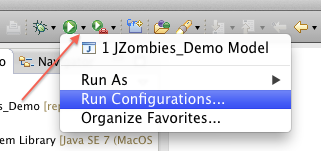
\includegraphics[width=3in]{images/zombies_launch.png}
}
\caption{JZombies Model Launcher}
\label{fig:launch}
\end{center}
\end{figure}

\section{The Batch Run Configuration GUI}
\label{sec:gui}
The  Batch Run Configuration GUI is used to configure and launch the batch run. To start the configuration GUI, start the JZombies demo model (see section \ref{sec:launch_model}) and click on the lightning bolt in the toolbar (fig. ~\ref{fig:gui_launch}). Note that you can also start the GUI as a stand-alone application. See section \ref{sec:gui_launch} for the details.

\begin{figure}[h]
\begin{center}
\vspace{.2in}
\centerline {

\includegraphics[width=3in]{images/gui_launch.png}
}
\caption{Batch Run Configuration GUI Launch}
\label{fig:gui_launch}
\end{center}
\end{figure}

The GUI is used to configure a batch run. This configuration can be saved and then loaded at a future time. The configuration GUI consists of a tool bar and four tabbed panels (fig. ~\ref{fig:config_gui}). The first four toolbar buttons 
\includegraphics[height=.2in]{images/gui_file_buttons.png} are used to create a new configuration, open an existing configuration, save the current configuration, and save the current configuration in a new file. Hovering over the buttons with the mouse will show a tooltip explaining the buttons function.  The fifth button 
\includegraphics[height=.2in]{images/reload_button.png} will reload the properties in the model panel from the current model. 

\begin{figure}[h]
\begin{center}
\vspace{.2in}
\centerline {
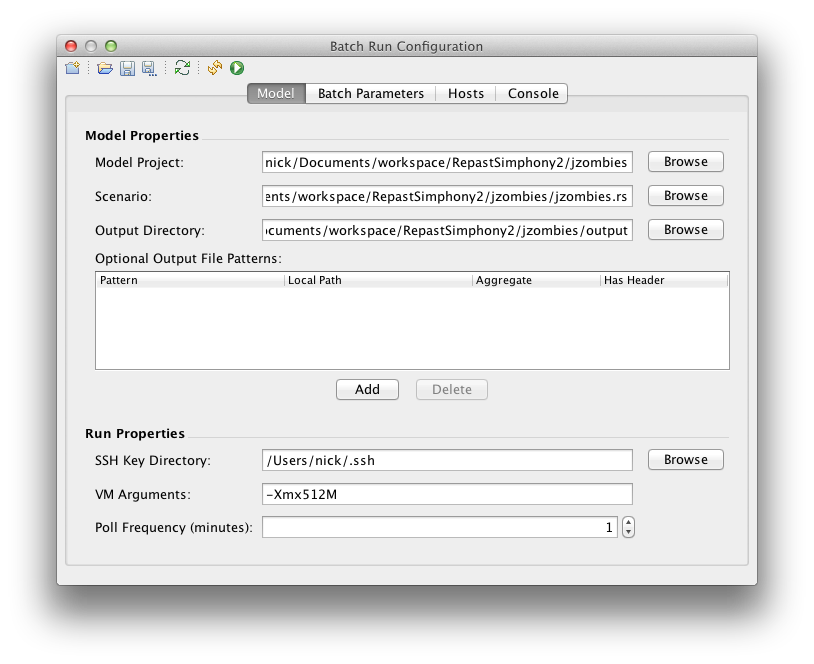
\includegraphics[width=6in]{images/config_gui.png}
}
\caption{Batch Run Configuration GUI}
\label{fig:config_gui}
\end{center}
\end{figure}


The remaining two buttons have to do with performing the batch runs itself. Regardless of type of batch run (local, distributed, and so forth), the batch run requires enough of Repast Simphony as well as the model to be run in order to work. These parts are bundled into a ``payload'' archive file that is then run locally or transferred to another machine depending on whether the runs are local or to be distributed among remote machines. The second to last button 
\includegraphics[height=.2in]{images/create_archive_button.png} will create this payload archive file for the current configuration. The last button  
\includegraphics[height=.2in]{images/run_button.png} will then execute the batch run.

\subsection{Model Panel}
When the batch configuration GUI is started and you have a model loaded in the Repast Simphony runtime then the GUI will create a new configuration with that model loaded. The model panel will contain various required model properties:

\begin{description}
\item[Model Project] The location of the project that contains the model. 
\item[Scenario] The location of the scenario directory of the model. 
\item[Output Directory] The directory where the model batch run output will be written.
\end{description}

The browse button next to each of these items can be used to select the directory for each property. The reload button
\includegraphics[height=.2in]{images/reload_button.png}  will load best guess defaults for these properties when the GUI is launched with an associated project.

The Run Properties sections defines properties that are used during the actual model run. 

\begin{description}
\item[SSH Key Directory] The directory that contains the user's public ssh rsa key. See the distributed runs section (section \ref{sec:distributed_runs}) below for more details.
\item[VM Arguments] The virtual machine arguments to use when performing the actual model runs.
\item[Poll Frequency] The frequency with which the master process will poll its clients to determine if they have finished.\end{description}

\subsection{Batch Parameters Panel}
The batch parameters panel (fig. ~\ref{fig:batch_params})  is used to define the parameter space that the batch run will iterate over. 

\begin{figure}[h]
\begin{center}
\vspace{.2in}
\centerline {
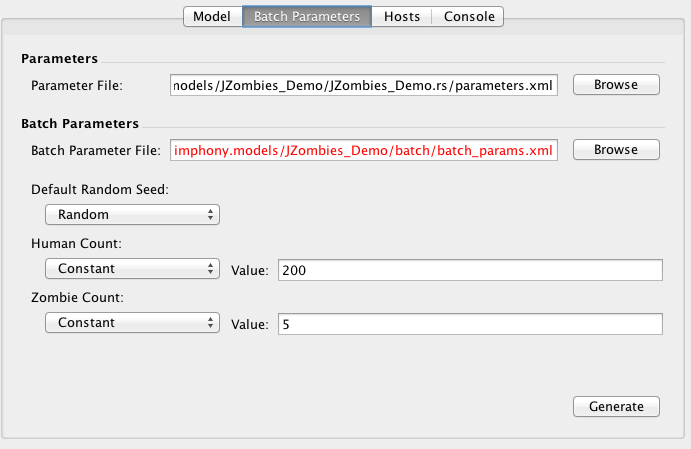
\includegraphics[width=6in]{images/batch_params_panel.png}
}
\caption{Batch Parameters Panel}
\label{fig:batch_params}
\end{center}
\end{figure}

\noindent It has two file properties.

\begin{description}
\item[Parameter File] The location of the non-batch parameter file for the model. This is typically the parameters.xml file in the scenario directory.
\item[Batch Parameter File] The location of the batch parameter file. By default, this will be the batch\_params.xml file the model's batch directory.
\end{description}

The GUI will use the parameters file to generate some sample batch parameters if the batch parameters file is empty. The parameters file is also used during the actual runs and thus the parameters in the non-batch parameters file must match those in the batch parameters file. Beneath the batch parameter file text box, you will see the actual parameters themselves. If the batch parameter file is empty, then the GUI will display the parameters in the parameter file as constant values. The drop down combo box underneath each parameter name can be used to define the value or range of values for that parameter during a batch run. The possible parameter types are:

\begin{description}
\item[Constant] The parameter will be set to the specified value in the ``value'' box and this value will remain constant over all the batch runs.
\item[Number Range] The parameter will begin at the value specified in the ``From'' text box and be incremented by the ``Step'' amount up to and including the ``To'' amount. 
\item[Space Separated List] The parameter will be set to each individual value in the ``Values'' list. The values should be space separated.
\item[Random] Sets the value at random. This only applies to the Random Seed which will then be initialized with the current time.
\end{description}

The full combination of the parameters defines the parameter space. The batch runs will iterate over the entire space. For example, if the 
Random Seed is set to a constant of 1, the Human Count to a Number Range where From: 1, To: 3, Step: 1 and the Zombie Count is set to a Space Separated List of ``20 15'', then the parameters for each run will be:

\begin{enumerate}
\item: Random Seed: 1, Human Count: 1, Zombie Count: 20
\item: Random Seed: 1, Human Count: 2, Zombie Count: 20
\item: Random Seed: 1, Human Count: 3, Zombie Count: 20
\item: Random Seed: 1, Human Count: 1, Zombie Count: 15
\item: Random Seed: 1, Human Count: 2, Zombie Count: 15
\item: Random Seed: 1, Human Count: 3, Zombie Count: 15
\end{enumerate}

Note that order of the runs with respect to the parameters may actually differ, but all the parameter combinations will be executed.

When the batch parameters as recorded in the batch parameter do not match the ones specified in the GUI, then the batch parameter file will be displayed in red.  (This will occur when a parameter type or value is changed.) The red indicates that the batch parameter file needs to be re-generated using the ``Generate'' button in the lower right of the panel.

\subsection{Hosts Panel}
The Hosts panel (fig. ~\ref{fig:hosts_panel}) is used to define the machines on which the batch runs will be performed. Both local and remote hosts can be defined. The left hand side of the panel lists the hosts that been previously defined (e.g. ``nick@localhost'') and the right hand side ``Host Properties'' displays the properties for the host selected on the left hand side. New hosts can be created using the ``Add Host'' 
\includegraphics[height=.2in]{images/add_host.png} button. A copy of an existing host can be made with the ``Copy Host'' 
\includegraphics[height=.2in]{images/copy_host.png} button. Existing hosts can be deleted by selecting the host to delete and pressing the ``Delete Host'' 
\includegraphics[height=.2in]{images/delete_host.png} button.

\begin{figure}[h]
\begin{center}
\vspace{.2in}
\centerline {
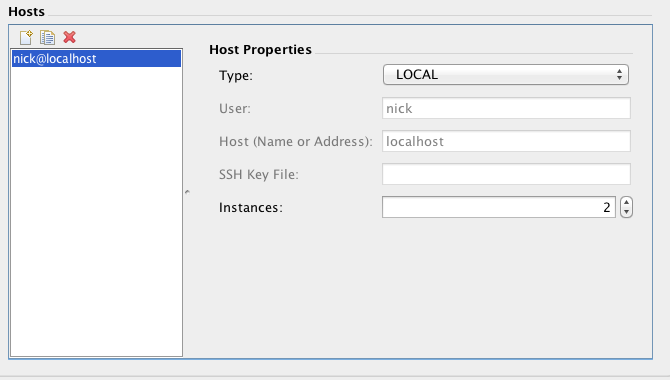
\includegraphics[width=6in]{images/hosts_panel.png}
}
\caption{Hosts Panel}
\label{fig:hosts_panel}
\end{center}
\end{figure}

The Host Properties are:

\begin{description}
\item[Type] The type of host: local or remote.
\item[User] The user name of the account on the remote machine. This is only used for a remote host.
\item[Host] The name or ip address of the remote machine. This is only used for a remote host.
\item[SSH Key File] The name of the private SSH key file used to auto-login on the remote host. This is only used for a remote host.
\item[Instances] The number of instances to run on the host. Each instance will be assigned a chunk of the parameter space to run.
\end{description}

Each of the hosts defined on the host panel will be used to perform the batch runs. For example, if one local host and one remote host is defined and the local host has two instances and the remote host has a single instance, then the batch parameter space will be divided in thirds. Two-thirds will be run locally in parallel: each instance on the local machine will run a third of the space. The remaining third will be run on the remote machine. The number of instances to run on a machine should be roughly the number of hardware threads available on the machine. Of course, your milage may vary, especially if the machine is performing other computationally expensive tasks.  

\subsubsection{Local Runs}
Local runs are the easiest runs to perform, requiring the least amount of external setup. To configure a local run, create a host (or chose an existing one) and set its type to LOCAL. You will see the host labeled as something like X@localhost where X is the user name of the account running the GUI. When you perform a local run, the GUI copies the archive payload mentioned above to a temporary location on the machine's hard-drive. This payload is unzipped and the parameter space is divided among the instances to be run locally and the runs are begun. Once the runs have ended, the output generated by each instance is concatenated together and placed in the output directory specified in the model panel.

\subsubsection{Remote Runs}
\label{sec:distributed_runs}
Remote runs are more complicated and you may have to do some setup on the local and remote machine. Remote machines can be anything from miscellaneous spare machines that you might have up to amazon's cloud computing services. Remote runs work over Secure Shell (SSH). SSH is a cryptographic network protocol for secure data communication, remote shell services or command execution and other secure network services between two networked computers that connect, via a secure channel over an insecure network, a server and a client (running SSH server and SSH client programs, respectively). Any machine that allows you to connect to it via SSH and can run a java virtual machine can be used to perform a remote run. See section \ref{sec:remote_machines} on how to set up the remote machines.

On the local side, that is, on the machine you are running the batch configuration GUI on, you will need to be setup to auto-login to the remote machine using public key authentication. This consists of creating a ssh public / private key pair on your machine, if those don't already exist, copying that key to the remote machine and then appending the key to the list of authorized keys on the remote machine. Some useful references that describe this are:

\begin{itemize}
\item OSX - \href{http://smbjorklund.no/ssh-login-without-password-using-os-x}{http://smbjorklund.no/ssh-login-without-password-using-os-x}
\item Windows - See below.
\item Linux - \href{https://hkn.eecs.berkeley.edu/~dhsu/ssh_public_key_howto.html}{https://hkn.eecs.berkeley.edu/$\sim$dhsu/ssh\_public\_key\_howto.html}
\end{itemize}

\noindent
Other sites exist as well,  google ``ssh public key authentication'' for more information.

The situation on windows is more complicated. OSX and Linux come with ssh and thus the built-in ability to generate public / private key pairs. Unfortunately, this is not the case for Windows and thus some setup is required. The following steps describe one way to generate the key pair and copy it to the remote machine under Windows.

\begin{enumerate}
\item Download and install the Git Client from \href{http://git-scm.com/download/win}{http://git-scm.com/download/win}.
\item From the start menu, run ``Git Bash''. You may need to navigate to the Git folder in "All Programs". Git Bash is terminal program in which you can type the commands to create the key pairs.
\item Check if you have a key pair already generated. If the files id\_rsa and id\_rsa.pub exist in an .ssh directory in your home directory (e.g. C:\textbackslash Users\textbackslash nick\textbackslash .ssh) then the keys already exist and you can skip to step 5.
\item In the Git Bash terminal type {\tt ssh-keygen -t rsa -C "your\_email@example.com"} We want the default settings so when asked to enter a file in which to save the key just press enter. Then enter a short passphrase. You should see see something like figure \ref{fig:win_ssh}
\item In the Git Bash terminal type {\tt scp \textasciitilde/.ssh/id\_rsa.pub user@machine:\textasciitilde} where user is the user name used to login to the remote machine and machine is the machine name or ip address. This will copy the public key into the home directory on the remote machine.
\item Login to the remote machine. Type {\tt ssh user@machine} replacing user and machine as appropriate. You will be asked for the password to login to the remote machine. 
\item Type {\tt cat id\_rsa.pub >> .ssh/authorized\_keys} to add the public key to the list of authorized keys on the remote machine. If you get a ``no such file or directory'' message, type {\tt mkdir .ssh; touch .ssh/authorized\_keys} and then  {\tt cat id\_rsa.pub >> .ssh/authorized\_keys} . If you get an error that .ssh already exists when trying to create the directory with {\tt mkdir}, type {\tt touch .ssh/authorized\_keys} and then  {\tt cat id\_rsa.pub >> .ssh/authorized\_keys} .
\item Type {\tt exit} to logout from the remote machine. 
\item Try to login to the remote machine again by typing {\tt ssh user@machine} replacing user and machine. If you are NOT asked for your password but are asked for your ssh private key passphrase then the setup was successful.
\end{enumerate}

\begin{figure}[h]
\begin{center}
\vspace{.2in}
\centerline {
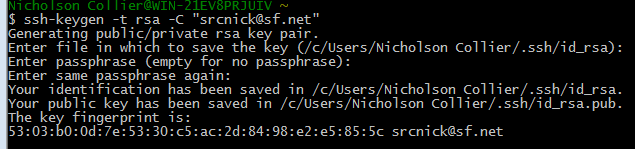
\includegraphics[width=6in]{images/win_ssh.png}
}
\caption{Key Generation with Git Bash}
\label{fig:win_ssh}
\end{center}
\end{figure}


Once you've got your keys on the remote machine, you can run remote batch runs using the Batch Run GUI. The host properties User, Host and SSH Key are used to login to the remote host. The User property should be the user name for the ssh login. The host is the name or ip address of the machine to login into and the SSH Key File is the private key file on the local machine used to auto-login to the remote machine. This file is typically called id\_rsa in a .ssh directory in the user's home directory,  but it may be different.

When performing a batch run using a remote host, the active payload will be copied to the account of the user specified in the host properties. After that, the run occurs as it does in the local version. The archive is unzipped and the parameter space is divided among the instances to be run on that remote host. When the instance runs have ended the output is copied back to the machine where the GUI was run, concatenated and written to the output directory.

\section{Preparing Your Model for Batch Runs}

The first requirement for a batch run is that your model must terminate each run. When running the model via the GUI this is typically done by clicking the stop button. In the batch run case, you must set and check some termination condition and then stop the model if that condition is met. Or, set the model to terminate at some specific tick. In the JZombies case, the first of these might look like:

\begin{verbatim}
if (context.getObjects(Human.class).size() == 0) {
   RunEnvironment.getInstance().endRun();
}
\end{verbatim}
\noindent
This checks to see if there are any more Humans and if not then it calls RunEnvironment to end the run. Context here is the model's master context. Something like this could be scheduled to execute once every tick either manually or via a scheduled method on the context builder.

The second option looks like:

\begin{verbatim}
RunEnvironment.getInstance().endAt(30);
\end{verbatim}
\noindent
This schedules the simulation to end at tick 30. It can be placed in the ContextBuilder for your model.

The second requirement concerns the model's file output. The batch mechanism assumes that the output is captured using Repast Simphony's File Sinks and that the files will be written somewhere within ``instance'' directory where the model runs. The best way to insure that this occurs to specify a file with a relative rather than absolute path in the File Sink Editor. In order to specify a relative path make sure that the file name does not begin with a ``/'' (under OSX, Linux) or ``X:\textbackslash'' or ``\textbackslash'' (under windows where X is any drive letter). The name can be anything and include subdirectories but the path must be relative. Figure ~\ref{fig:file_name} is an example of a relative path.

\begin{figure}[h]
\begin{center}
\vspace{.2in}
\centerline {
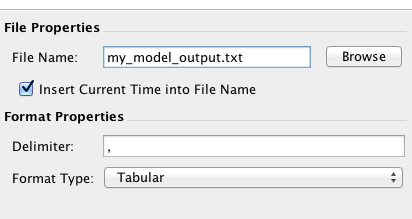
\includegraphics[width=6in]{images/file_name.png}
}
\caption{Relative Path in File Sink Editor}
\label{fig:file_name}
\end{center}
\end{figure}

\section{Batch Run Model Output}
As mentioned above the output from each instance will be concatenated and copied into the output directory specified in the GUI. The file sink output will look the same as a normal non-batch run except that the run numbers will likely not be in numeric order given that the concatenation makes no account for order. For example, the output from run 11 may appear before that from run 2.

\begin{verbatim}
"run","tick","Human Count","Zombie Count"
1,0.0,200,5
1,1.0,200,5
...
11,0.0,220,15
11,1.0,220,15
11,2.0,209,26
...
2, 0.0, 12, 200
...
\end{verbatim}

For each file sink output there will be a batch param map text file that specifies the batch parameters that were used to initialize that run. For example,

\begin{verbatim}
"run","randomSeed","human_count","zombie_count"
1,1,200,5
11,1,220,15
2,1,250,5
\end{verbatim}

Here run 1 was initialized with a random seed of 1, a human count of 200 and zombie count of 5. Run 11 was initialized with a random seed of 1 a human count of 220 and zombie count of 15.

You will also see a status\_output.properties file in the output directory. This reports the final status of each local and remote instance. For example,

\begin{verbatim}
ec2-107-20-23-221.compute-1.amazonaws.com.ubuntu.1 = OK
ec2-107-20-23-221.compute-1.amazonaws.com.ubuntu.2 = OK
localhost.nick.1 = OK
\end{verbatim}
\noindent
The format here is ``hostname.username.instance number = status".  In this case, we ran two instances on an amazon cloud machine with the name of ec2-107-20-23-221.compute-1.amazonaws.com under the ubuntu user. Both those finished successfully. We also ran one instance on the localhost under the nick user. That finished successfully as well. When the runs don't finish successfully you will see status other than ``OK'', such as ``FAIL''. There will also be additional log files in the output directory containing some details on the failure.


\section{An Example}
This section will walk you through an example batch run using a combination of local and remote machines. We will run 1 instance locally, 2 instances on a remote OSX machine and 1 instance on an Amazon EC2 cloud instance. We have set up the remote OSX machine and the Amazon cloud host using the instructions in section \ref{sec:remote_machines}. The JZombies demo will be our example model.

We've set up the Model, Batch Parameters and Hosts Panel as in fig. ~\ref{fig:model_panel_run}, fig. ~\ref{fig:batch_panel_run} and fig. ~\ref{fig:hosts_panel_run} respectively. Note that the IP address of the OSX machine as been obscured. If you want to follow along with the example, fill the Run Properties part of the Model panel as in the figure and set the batch parameters in the Batch Parameters panel to match the batch panel figure. For the hosts, create only a local host with two instances. To do that, go to the hosts panel, if there is an existing localhost entry, click on it and make sure the instances entry is 2. If there is no localhost entry, click the ``Add Host'' 
\includegraphics[height=.2in]{images/add_host.png} button and set its type to LOCAL and instances to 2. 

\begin{figure}[h]
\begin{center}
\vspace{.2in}
\centerline {
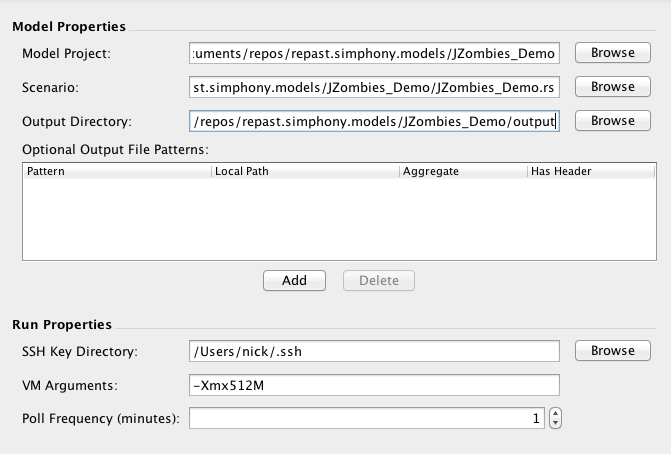
\includegraphics[width=6in]{images/model_panel_run.png}
}
\caption{Model Panel For Run}
\label{fig:model_panel_run}
\end{center}
\end{figure}

\begin{figure}[h]
\begin{center}
\vspace{.2in}
\centerline {
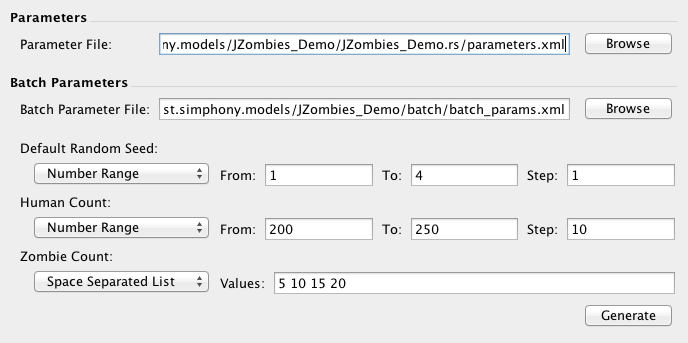
\includegraphics[width=6in]{images/batch_panel_run.png}
}
\caption{Batch Panel For Run}
\label{fig:batch_panel_run}
\end{center}
\end{figure}

\begin{figure}[h]
\begin{center}
\vspace{.2in}
\centerline {
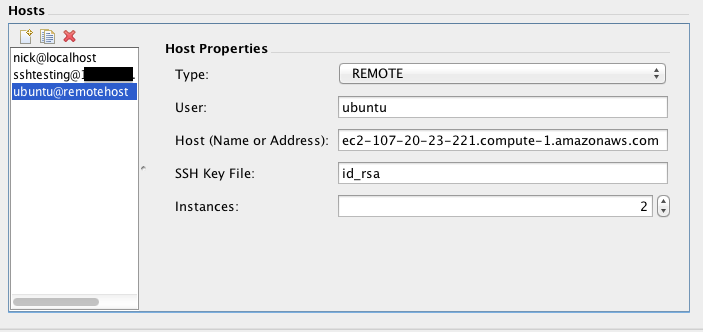
\includegraphics[width=6in]{images/hosts_panel_run.png}
}
\caption{Hosts Panel For Run}
\label{fig:hosts_panel_run}
\end{center}
\end{figure}


Once the various configuration properties have been set, we can click the run button. This will create the archive payload and start the runs. The Console panel will display information about the archive creation and then about the runs themselves. If you have a passphrase associated with your SSH key and you are doing remote runs you will be asked for  your passphrase in the passphrase dialog (fig. ~\ref{fig:passphrase}). 

The Console output reports the status of the batch run from setup through the actual runs. It can look daunting at first but it contains lots of useful information. Much of the output begins with a status keyword such as INFO, WARN or ERROR. If the run completes without any issues you should see only INFO type status messages. Following the status keyword is a timestamp followed by the name of the Java class that is producing the status message. After that, you will see the status message itself.

The first status message tells us that a ``config.props'' file has been written to the output directory. The config.props file
contains all the batch run properties that were entered into the GUI. The code that performs the batch runs reads this config file and performs the runs using that information. (In what follows, the file paths have been shortened for formatting purposes.  You will see the full file path).

\begin{verbatim}

INFO  [AWT-EventQueue-0] 16:55:18,582 
  repast.simphony.batch.gui.BatchConfigMediator - Writing batch 
  run config file to: JZombies_Demo/output/config.props
\end{verbatim}

The second status message says that the batch\_params.xml file that was created via the GUI is ``unrolled'' and written to a temporary directory. ``Unrolling'' here refers to explicitly producing and writing each individual parameter combination to a file. It is this unrolled parameter file that is divided and distributed to the hosts for running. 

\begin{verbatim}
INFO  [AWT-EventQueue-0] 16:55:18,588 
  repast.simphony.batch.gui.BatchConfigMediator - 
  Unrolling batch parameter file: JZombies_Demo/batch/batch_params.xml to
  /var/folders/31/yd0l22kx35zgy1wbnc8p7gbr0000gr/T/unrolledParamFile.txt
\end{verbatim}

The next section is the output of the Ant script (see \href{http://ant.apache.org}{http://ant.apache.org}) that creates the archive payload. Here we can see the creation of a working directory underneath a temporary directory. This working directory will contain the model itself and the Repast Simphony code necessary to run the model.  The [copy] and [jar] sections report model code and files being copied into the working directory and the creation of jar archives containing the necessary repast code. (I've replaced part of the temporary path with ``...'' and truncated the jar section a bit to improve the readability here.)

\begin{verbatim}
make_zip:
   [delete] Deleting directory /private/var/folders/.../working
   [mkdir] Created dir: /private/var/folders/.../working
   [mkdir] Created dir: /private/var/folders/.../working/bin
   [mkdir] Created dir: /private/var/folders/.../working/scenario.rs
   [copy] Copying 2 files to /private/var/folders/.../working
   [copy] Copying 3 resources to /private/var/folders/.../working
   [copy] Copying 1 resource to /private/var/folders/.../working/bin
 
make_pre_reqs:
    [mkdir] Created dir: /private/var/folders/.../working/data
    [mkdir] Created dir: /private/var/folders/.../working/lib
    ...
    [jar] Building jar: /private/var/folders/.../working/lib/repast.simphony.batch.jar
    [jar] Building jar: /private/var/folders/.../working/lib/repast.simphony.statecharts.jar
    [copy] Copying 69 files to /private/var/folders/.../working/lib
    [jar] Building jar: /private/var/folders/.../working/lib/model.jar
    [copy] Copying 10 files to /private/var/folders/.../working/scenario.rs
    [move] Moving 1 file to /private/var/folders/.../working/scenario.rs

     [jar] Building jar: JZombies_Demo/output/complete_model.jar
     [echo] Completed building model archive.
\end{verbatim}

The archive payload is then copied to the local and remote hosts. The process here is that a zip archive is created containing the archive payload as well as some additional configuration data. This zip archive is named with the user name followed by the host together with a timestamp (e.g. nick\_localhost4106394375716993975.zip). In the case of a local host, the zip archive is copied to a local temporary directory whose name begins with simphony\_model\_ followed by a timestamp (e.g. simphony\_model\_1368219324898). 

\begin{verbatim}
INFO  [SwingWorker-pool-1-thread-2] 16:56:26,990 
  repast.simphony.batch.ssh.LocalSession - 
  Copying locally /var/folders/.../nick_localhost4106394375716993975.zip
  to  /var/folders/.../simphony_model_1368219324898
INFO  [SwingWorker-pool-1-thread-2] 16:56:27,411 
  repast.simphony.batch.ssh.LocalSession - Copying Finished.
\end{verbatim}

The remote host works similarly. The zip archive is copied to a simphony\_model\_ plus timestamp directory on the remote host. In this case, the zip archive is named  ubuntu\_ec2-107-20-23-221.compute-1.amazonaws.com8807870753490178805.zip and the remote directory is ~/simphony\_model\_1368219324898/.

\begin{verbatim}
INFO  [SwingWorker-pool-1-thread-2] 16:56:09,829 
  repast.simphony.batch.ssh.RemoteSession - 
  Copying /var/folders/.../
  ubuntu_ec2-107-20-23-221.compute-1.amazonaws.com8807870753490178805.zip to 
  ubuntu@ec2-107-20-23-221.compute-1.amazonaws.com:~/simphony_model_1368219324898/
  ubuntu_ec2-107-20-23-221.compute-1.amazonaws.com8807870753490178805.zip ...
INFO  [SwingWorker-pool-1-thread-2] 16:56:23,197 
  repast.simphony.batch.ssh.RemoteSession - Copying Finished.
\end{verbatim}

Before a remote run is attempted,  a check is made to see if Java is installed on the remote host. If it is not, then you will see an error. In this case, we can see that the java version is 1.7.0\_21.

\begin{verbatim}
INFO  [SwingWorker-pool-1-thread-2] 16:56:33,369 
  repast.simphony.batch.ssh.RemoteSession - 
  Checking for java on ubuntu@ec2-107-20-23-221.compute-1.amazonaws.com
INFO  [Connect thread ec2-107-20-23-221.compute-1.amazonaws.com session] 16:56:33,691
  repast.simphony.batch.ssh.SSHSession - java version "1.7.0_21"
INFO  [Connect thread ec2-107-20-23-221.compute-1.amazonaws.com session] 16:56:33,692
  repast.simphony.batch.ssh.SSHSession - OpenJDK Runtime Environment (IcedTea 2.3.9)
  (7u21-2.3.9-0ubuntu0.11.10.1)
INFO  [Connect thread ec2-107-20-23-221.compute-1.amazonaws.com session] 16:56:33,692 
  repast.simphony.batch.ssh.SSHSession - 
  OpenJDK 64-Bit Server VM (build 23.7-b01, mixed mode)
\end{verbatim}

Once the java version has been checked and assuming it is OK, then the archive payload is unzipped and run.

\begin{verbatim}
INFO  [SwingWorker-pool-1-thread-2] 16:56:38,685 
  repast.simphony.batch.ssh.LocalSession - Unzipping model 
  /var/folders/.../simphony_model_1368219324898/nick_localhost4106394375716993975.zip
INFO  [SwingWorker-pool-1-thread-2] 16:56:39,177 
  repast.simphony.batch.ssh.LocalSession - Running model on localhost ...

INFO  [SwingWorker-pool-1-thread-2] 16:56:34,583 
  repast.simphony.batch.ssh.RemoteSession - Unzipping model on 
  ubuntu@ec2-107-20-23-221.compute-1.amazonaws.com
INFO  [SwingWorker-pool-1-thread-2] 16:56:37,633 
 repast.simphony.batch.ssh.RemoteSession - Running model on 
 ubuntu@ec2-107-20-23-221.compute-1.amazonaws.com ...
\end{verbatim}

The remote and local hosts are then periodically polled to see if they have finished. The polling status updates end with ``DONE:'' followed by a ``yes'' if the runs on that host have finished. Otherwise ``no'' will be output.

\begin{verbatim}
INFO  [pool-3-thread-3] 16:56:51,210 repast.simphony.batch.ssh.LocalDonePoller - 
  Polled /var/folders/.../simphony_model_1368219324898 for DONE:  yes
INFO  [pool-3-thread-2] 16:56:52,540 repast.simphony.batch.ssh.RemoteDonePoller - 
 Polled simphony_model_1368219324898 on ec2-107-20-23-221.compute-1.amazonaws.com 
 for DONE: yes
INFO  [pool-3-thread-1] 16:56:52,796 repast.simphony.batch.ssh.RemoteDonePoller - 
  Polled simphony_model_1368219324898 on XXX.XXX.XXX.XXX 
  for DONE: yes
\end{verbatim}

If there was error during the run, that should be reported here as part of the polling. Assuming there wasn't then the local and remote output is copied and concatenated into the output directory that was specified in the GUI.

\begin{verbatim}
INFO  [SwingWorker-pool-1-thread-2] 16:56:55,630 
  repast.simphony.batch.ssh.RemoteSession - Finding and copying remote 
  output from sshtesting@XXX.XXX.XXX.XXX:simphony_model_1368219324898 
  to /var/folders/.../sshtesting_XXX.XXX.XXX.XXX
INFO  [SwingWorker-pool-1-thread-2] 16:56:58,412 
  repast.simphony.batch.ssh.RemoteSession - Finding and copying remote
  output from ubuntu@ec2-107-20-23-221.compute-1.amazonaws.com:
  simphony_model_1368219324898 to /var/folders/.../
  ubuntu_ec2-107-20-23-221.compute-1.amazonaws.com
INFO  [SwingWorker-pool-1-thread-2] 16:57:00,247 
  repast.simphony.batch.ssh.LocalSession - Finding output on localhost in
  /var/folders/.../simphony_model_1368219324898
INFO  [SwingWorker-pool-1-thread-2] 16:57:00,266 
  repast.simphony.batch.ssh.SessionsDriver - Aggregating output into 
  JZombies_Demo/output
INFO  [SwingWorker-pool-1-thread-2] 16:57:00,267 
  repast.simphony.batch.ssh.SessionsDriver - Finished. Elapsed Time: 1.5906
\end{verbatim}

\begin{figure}[h]
\begin{center}
\vspace{.2in}
\centerline {
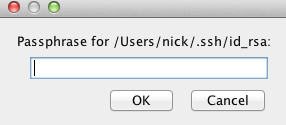
\includegraphics[width=3in]{images/passphrase.png}
}
\caption{Passphrase Dialog}
\label{fig:passphrase}
\end{center}
\end{figure}


\section{Remote Machine Setup}
\label{sec:remote_machines}

In order to perform a run on a remote machine that machine must be set up to accept an ssh connection and you must have an account on the remote machine. Once the remote machine has been setup for ssh logins, you then need to add your public key to its authorized\_keys file as described in section \ref{sec:distributed_runs}. The remote machine must have Java 7 installed and it must be be the default Java.

\subsection{OSX }
Allowing remote logins on OSX is done using the System Preferences on the machine you want to remotely login to. Start System Preferences and double click on the sharing icon. Select the Remote Login as seen in figure \ref{fig:osx_sys}. Make sure you allow access for the user you will be logging in as. You should now be able to ssh into the remote machine and copy your public keys to the server as described in links given in section \ref{sec:distributed_runs}.

\begin{figure}[h]
\begin{center}
\vspace{.2in}
\centerline {
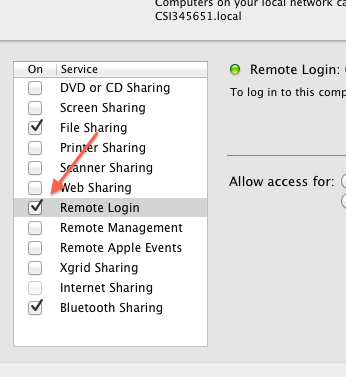
\includegraphics[width=3in]{images/sshd_on_osx.png}
}
\caption{Enabling SSHD on OSX}
\label{fig:osx_sys}
\end{center}
\end{figure}

\subsection{Linux / Unix}
Chances are if the remote machine is running Linux or another Unix variant it is already set up to allow ssh logins. If not, follow your distributions instructions for turning on the sshd service. You should now be able to ssh into the remote machine and copy your public keys to the server as described in section \ref{sec:distributed_runs}.

\subsection{Windows}

Windows does not come with a SSH server and so one must be provided. As a solution to this, we've provided a Virtual Box virtual machine running a linux distribution. You can run this on your windows machine and the remote batch runs will be performed on that. (Again, this  is only required to use a windows machine as a remote machine not to do local runs on a windows machine.)

\begin{enumerate}
\item Download and Install Virtual Box from \href{https://www.virtualbox.org/wiki/Downloads}{https://www.virtualbox.org/wiki/Downloads}.
\item Download Repast Simphony  virtual machine file (Repast\_VM\_Ubuntu\_12.0.4.ova) from \href{http://sourceforge.net/projects/repast/files/Repast\%20Simphony/Repast\%20Simphony\%202.1/Repast_VM_Ubuntu_12.0.4.ova/download}
{http://sourceforge.net/projects/repast/files/Repast \\
Simphony/Repast Simphony 2.1/Repast\_VM\_Ubuntu\_12.0.4.ova/download}
\item Double Click on the downloaded virtual machine. Virtual Box should start with the Import Virtual Appliance Dialog up (fig. \ref{fig:import_vm}).
\item Click the Import button to import the virtual machine.
\end{enumerate}

\begin{figure}[h]
\begin{center}
\vspace{.2in}
\centerline {
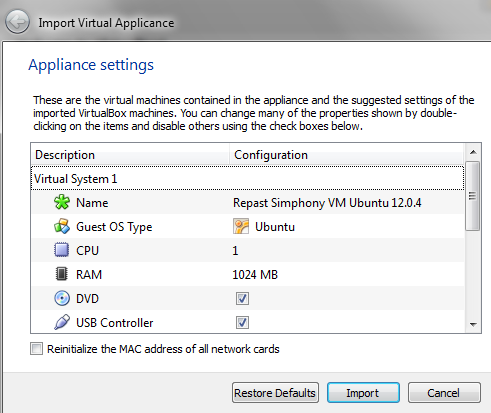
\includegraphics[width=4.5in]{images/import_vm.png}
}
\caption{Import the Repast Simphony Server Virtual Machine}
\label{fig:import_vm}
\end{center}
\end{figure}

\noindent
To run the virtual machine so that it can be used do the batch runs:

\begin{enumerate}
\item Start Virtual Box
\item Start the virtual machine. You should see it on the left hand side named Repast Simphony VM Ubuntu 12.0.4. (fig \ref{fig:vm}). Double click it. While the virtual machine is starting you will see some Virtual Box Information messages.
\item If you see an error message about network settings, click the ``Change Network Settings" button (fig. \ref{fig:network_error}) and then the OK button in the settings dialog that pops up.
\item The virtual machine will then run through its boot process (this may take a minute or two the first time) and eventually you will be presented with a command prompt (fig. \ref{fig:vm_login}). (The virtual machine is configured as a server without a GUI.)
\end{enumerate}

\begin{figure}[h]
\begin{center}
\vspace{.2in}
\centerline {
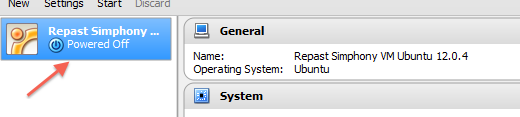
\includegraphics[width=4.5in]{images/vm.png}
}
\caption{Repast Simphony Server Virtual Machine}
\label{fig:vm}
\end{center}
\end{figure}

\begin{figure}[h]
\begin{center}
\vspace{.2in}
\centerline {
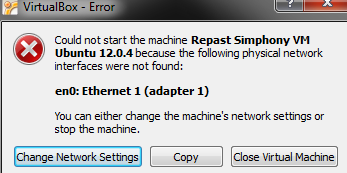
\includegraphics[width=4.5in]{images/network_error.png}
}
\caption{Network Error Dialog}
\label{fig:network_error}
\end{center}
\end{figure}

\begin{figure}[h]
\begin{center}
\vspace{.2in}
\centerline {
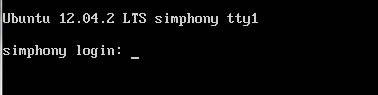
\includegraphics[width=4.5in]{images/vm_login.png}
}
\caption{VM Login}
\label{fig:vm_login}
\end{center}
\end{figure}

At this point, the virtual machine is almost ready to do the batch runs. You still need to (1) get the IP address of the virtual machine in order to connect to it, and (2) you need to copy your public key over to it. To find the IP address:

\begin{enumerate}
\item Boot the virtual machine, if you haven't already.
\item Login to the virtual machine using a username of {\tt simphony} and a password of {\tt simphony}.
\item Once logged in, you should see a welcome message that includes the ip address. It should say something like: {\tt IP Address for eth0: XXX.XXX.XXX.XXX} where the Xs are replaced with your IP address (fig. \ref{fig:ip}). Note that eth0 might also be different. You can also get the IP address by running the ifconfig command. You will see the details of all the installed network interfaces. These include an ``inet addr'' entry that specifies the ip address.
\end{enumerate}

\begin{figure}[h]
\begin{center}
\vspace{.2in}
\centerline {
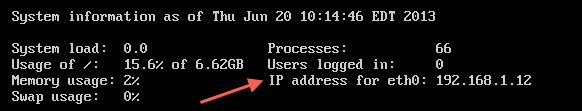
\includegraphics[width=5in]{images/ip.png}
}
\caption{IP Address}
\label{fig:ip}
\end{center}
\end{figure}

Once you have the IP address you can use that as the Host for batch runs. The user will again be {\tt simphony}. Lastly, you will still have to perform the one time copy of your public key to this machine as described in the Remote Runs section (section \ref{sec:distributed_runs}). Once that has been accomplished, the machine is ready. Note that you do not need to log directly into it, it only needs to be running. The default password is {\tt simphony}. If you want to change it, you can use the {\tt passwd}  command.

To shut down the virtual machine when you no longer need it, you can close the window as normal. This should pop up a Close Virtual Machine Dialog. Make sure the Send the shutdown signal is selected and then click OK.

\subsection{Amazon Cloud Services}
Amazon Elastic Compute Cloud (Amazon EC2) is a web service that provides resizable compute capacity in the cloud. It is designed to make web-scale computing easier for developers. It is possible to use this remote compute capacity to perform remote batch runs. More on Amazon's EC2 can be found at  \href{http://docs.aws.amazon.com/AWSEC2/latest/UserGuide/concepts.html}{http://docs.aws.amazon.com/AWSEC2/latest/UserGuide/concepts.html}.

Amazon EC2 based batch runs begin with setting up a remote machine instance that runs an Amazon Machine Image (AMI). The batch run will login into this instance using SSH and perform the runs on it. The setup only needs to be done once. After that, the instance can be stopped and started as needed. The Amazon EC2 Getting Started docs describe this process: \href{http://docs.aws.amazon.com/AWSEC2/latest/UserGuide/EC2_GetStarted.html}{\\http://docs.aws.amazon.com/AWSEC2/latest/UserGuide/EC2\_GetStarted.html}. (Note that Amazon, at the time of writing, has 12 month free tier. See the links in the EC2 Getting Started Guide for more info.) Follow the Getting Started Guide to set up your instance. Choose the 64 bit Ubuntu Server 12.04 LTS (figure \ref{fig:ubuntu_ami}) as the launch configuration in Step 2. of the Getting Started Guide. 

\begin{figure}[h]
\begin{center}
\vspace{.2in}
\centerline {
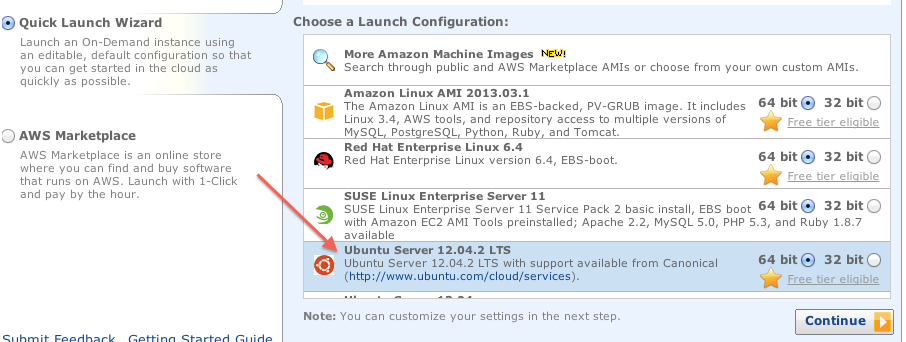
\includegraphics[width=6in]{images/ubuntu_ami.png}
}
\caption{Select the Ubuntu 12.04 AMI}
\label{fig:ubuntu_ami}
\end{center}
\end{figure}

Once your instance is running, log into and explore the instance as described in Step 3 and Step 4 of the Amazon Getting Started Guide. You do NOT need to attach an EBS volume, but you do need to install Java on the instance. From the command line that you should see after you've logged in, run the following commands (type them in and press enter after each one):

\begin{Verbatim}
sudo apt-get update
sudo apt-get install openjdk-7-jre-headless
sudo apt-get install zip
\end{Verbatim}

After each command, you may get a question about whether to continue with the install. Accept the default 'Yes' by pressing the enter key. Once you've done this, your instance should be ready to perform a batch run. The username to log in with is {\tt ubuntu} as is the password. To see the address of your instance, click on the instance in your EC2 Instances console. The host address for your batch configuration should appear in the instance details below it (figure \ref{fig:instance_addr}). If you do not see the instance address there, click on the refresh button (the circular arrow) in the upper right hand corner of the instance console. Make sure to stop your instance when you are done using it. When you restart the instance the next time, the address will have changed so be sure to update your batch configuration properties.

Amazon EC2 has its own public key authentication setup that is described in its Getting Started document. Consequently, the procedures described in section \ref{sec:distributed_runs} are not required here.

 \begin{figure}[h]
\begin{center}
\vspace{.2in}
\centerline {
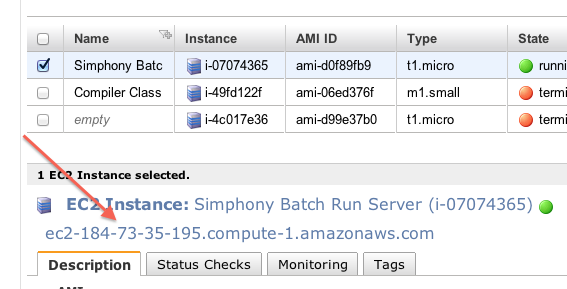
\includegraphics[width=6in]{images/instance_addr.png}
}
\caption{Instance Address}
\label{fig:instance_addr}
\end{center}
\end{figure}

\label{sec:gui_launch}
\section{Launching the Batch Run Configuration GUI} 
Batch Run Configuration GUI can be launched in 3 different ways. 

\begin{enumerate}
\item Using the Launch Button found in the runtime
\item Using the Eclipse Launcher in your project's launchers folder
\item Using the stand alone Batch Run applications
\end{enumerate}
\noindent
We have covered the first of these in section \ref{sec:gui}. The remaining two allow you to launch the configuration GUI and thus batch runs without launching the repast runtime. 

\subsection{Launching from Eclipse}
To launch the batch GUI from the eclipse launcher, open the launchers folder in your model's eclipse project and right click on the launch file that begins with ``Batch'' (fig \ref{fig:launcher}). Select ``Run As'' from the pop up menu and then the Batch model entry. This will launch the batch GUI and load the selected model into it. Note that when running via the launcher some of the output that would normally be in the Batch Run GUI Console will show up in Eclipse's console.

\begin{figure}[h]
\begin{center}
\vspace{.2in}
\centerline {
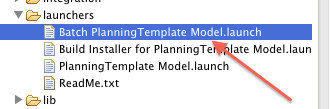
\includegraphics[width=6in]{images/batch_run_launcher.png}
}
\caption{Eclipse Launcher for Batch Run GUI}
\label{fig:launcher}
\end{center}
\end{figure}

\subsection{Launching as a Standalone Application}
To launch the batch GUI as a stand alone application navigate to where Repast Simphony is installed. On OSX, double click on the Batch Runner-1.0 application. On Windows or Linux, double click the batch\_runner.jar. 
 
\section{Running on a Cluster or HPC Machine}

It is also possible to perform batch runs on a cluster or a high performance computing (HPC) type machine. Such machine are composed of many processors each of which can run one or more batch run instances and all of which have access to a shared file system. Cluster / HPC runs will use the payload archive produced by the GUI  but are not themselves run via the GUI. These batch runs will use the job submission paradigm that is standard on these types of machines.

The first step for running a model on an HPC machine is to copy the payload complete\_model.jar to the remote machine. The payload is located in the model's output directory and can be created using the Batch Configuration GUI with the create archive button (
\includegraphics[height=.2in]{images/create_archive_button.png}). The transfer is often done via scp or similar secure copy methods. After copying the payload to the desired location, the next step is to unzip the payload:

\begin{verbatim}
unzip complete_model.jar
\end{verbatim}

We will be using the Portable Batch System (PBS) job scheduler for this example. This is a common job scheduler. If your system uses a different scheduler, it should be possible to adapt the instructions below. The first file to look at is the repast.pbs file. This is the file that is submitted to the PBS scheduler. The top section of the file looks like:
\begin{verbatim}
#!/bin/bash
#PBS -N <Job_Name>
#PBS -q <Queue_Name>
#PBS -l nodes=<nodes>:ppn=<ppn>
#PBS -m e
\end{verbatim}

\noindent where the elements in the angled brackets are meant to be edited for each individual use case. So, for example, if we wanted to name the job ``Zombies\_Test", submit the job to the ``shared" queue,  use 2 nodes and 8 processors per node we might issue the following \texttt{sed} command, all one line:
\begin{verbatim}
sed -i -e 's/<Job_Name>/Zombies_Test/' -e 's/<Queue_Name>/shared/'
-e 's/<nodes>/2/' -e 's/<ppn>/8/' repast.pbs
\end{verbatim}
Alternatively the repast.pbs file can be edited by hand. The particulars for each system may be slightly different so you may need to consult with the reference manual or online help of the system you will be using.

The next step is to make sure that all the scripts are executable by issuing the command:
\begin{verbatim}
chmod +x *.sh
\end{verbatim}
At this point the job is ready for submission and can be submitted via the command:
\begin{verbatim}
qsub repast.pbs
\end{verbatim}

The job is submitted to the specified queue and will run when the scheduler decides to run the job. Depending on the particular setup of the scheduler, you may receive an email alert when the job has finished running. Whichever method you use to figure out when the job has completed executing, you can run an output combiner to combine the data output from the individual simulations that were run with the command:
\begin{verbatim}
./outputcombiner.sh
\end{verbatim}
The combines data will be placed in a combined\_data directory in the current directory.



\end{document}  